\begin{frame}
  \frametitle{Introduction and Procedure}
  \begin{columns}
        \column[t]{5cm}
        Many of the new advanced reactors will use \gls{HALEU} fuel. 
        What are the resource requirements to meet expected \gls{HALEU}
        demand?

        \begin{block}{Procedure}
            Modeled three fuel cycle scenarios using \Cyclus
            \begin{itemize}
                \item Scenario 1: Current fleet of \glspl{LWR}
                \item Scenario 2: No growth transition to \gls{USNC} \gls{MMR}
                \item Scenario 3: No growth transition to X-energy Xe-100
            \end{itemize}
 
        \end{block}
        
        \column[t]{6cm}
        \begin{figure}[t]
            \begin{center}
            \begin{tikzpicture}[node distance=0.7cm, scale=0.8]
                \node (mine) [facility] {\tiny Uranium Mine};
                \node (mill) [facility, below of=mine] {\tiny  Uranium Mill};
                \node (conversion) [facility, below of=mill] {\tiny  Conversion};
                \node (enrichment) [facility, below of=conversion, xshift=-1.5cm]{\tiny Enrichment};
                \node (enrichment2) [transition, below of=conversion, xshift=1.5cm]{\tiny  Enrichment};
                \node (fabrication2) [transition, below of=enrichment2,yshift=-0.75cm]{\tiny Fuel Fabrication};
                \node (fabrication) [facility, below of=enrichment, yshift=-0.75cm]{\tiny Fuel Fabrication};
                \node (reactor) [facility, below of=fabrication]{\tiny Reactor};
                \node (adv_reactor) [transition, below of=fabrication2]{\tiny Advanced Reactor};
                \node (wetstorage) [facility, below of=reactor]{\tiny  Wet Storage};
                \node (drystorage) [facility, below of=wetstorage]{\tiny Dry Storage};
                \node (sinkhlw) [facility, below of=drystorage, xshift=1.5cm]{\tiny  HLW Sink};
                \node (sinkllw) [facility, below of=enrichment, xshift=1.5cm]{\tiny  LLW Sink};
        
                \draw [arrow] (mine) -- node[anchor=east]{\tiny Natural U} (mill); 
                \draw [arrow] (mill) -- node[anchor=east]{\tiny U$_3$O$_8$}(conversion); 
                \draw [arrow] (conversion) -- node[anchor=east]{\tiny UF$_6$}(enrichment);
                \draw [arrow] (enrichment) -- node[anchor=east]{\tiny Enriched U}(fabrication);
                \draw [arrow] (conversion) -- node[anchor=east]{\tiny UF$_6$}(enrichment2);
                \draw [arrow] (enrichment2) -- node[anchor=west]{\tiny HALEU}(fabrication2);
                \draw [arrow] (enrichment) -- node[anchor=east]{\tiny Tails}(sinkllw);
                \draw [arrow] (enrichment2) -- node[anchor=west]{\tiny Tails}(sinkllw);
                \draw [arrow] (fabrication) -- node[anchor=east]{\tiny Fresh UOX}(reactor);
                \draw [arrow] (fabrication2) -- node[anchor=west]{\tiny TRSIO fuel}(adv_reactor);
                \draw [arrow] (reactor) -- node[anchor=east]{\tiny Spent UOX}(wetstorage);
                \draw [arrow] (wetstorage) -- node[anchor=east]{\tiny Cool Spent UOX}(drystorage);
                \draw [arrow] (drystorage) -- node[anchor=east]{\tiny Casked Spent UOX}(sinkhlw);
                \draw [arrow] (adv_reactor) -- node[anchor=west]{\tiny Spent TRISO Fuel}(sinkhlw);
        
            \end{tikzpicture}
            \caption{Material flow of fuel cycle scenarios}
            \label{fig:fuel_cycle}
            \end{center}
        \end{figure}
        

  \end{columns}
        
\end{frame}

\begin{frame}
\frametitle{Results}
    \begin{columns}
        \column[t]{5cm}
        \begin{figure}[t]
            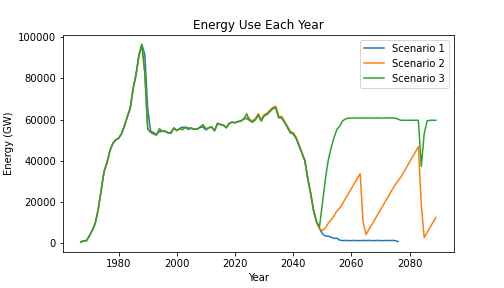
\includegraphics[scale=0.26, trim=0 5 0 10,clip]{figures/energy_all.png}
            \caption{Total Energy output of each scenario}
            \label{fig:energy}
        \end{figure}
        \begin{figure}[ht]
            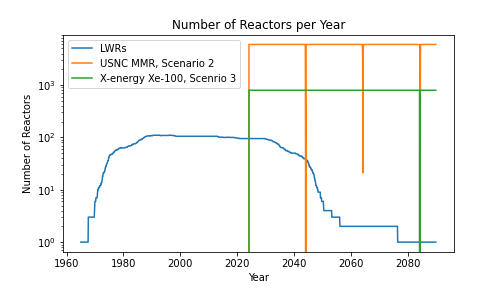
\includegraphics[scale=0.26, trim=0 5 0 10,clip]{figures/rx_deployment_all.png}
            \caption{Total Energy output of each scenario}
            \label{fig:ex_deployment}
        \end{figure}

        \column[t]{5cm}
    \begin{figure}[ht]
        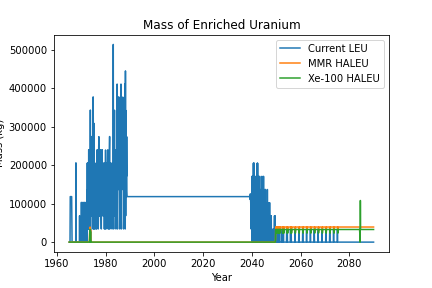
\includegraphics[scale=0.25,trim=0 5 0 10,clip]{figures/enrichedU_all.png}
        \caption{Total Energy output of each scenario}
        \label{fig:enrichedU}
    \end{figure}
    \begin{figure}[ht]
        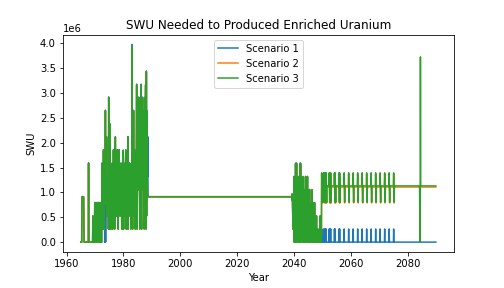
\includegraphics[scale=0.25,trim=0 5 0 10,clip]{figures/swu_all.png}
        \caption{Total Energy output of each scenario}
        \label{fig:swu}
    \end{figure}
    
        
        

    \end{columns}


\end{frame}

\begin{frame}
\frametitle{Conclusions}
    \begin{itemize}
        \item Scenario 2 required a higher mass of \gls{HALEU}
        \item Scenario 3 required more \gls{SWU}
    \end{itemize}

    \begin{block}{Ongoing Work}
        \begin{itemize}
            \item Adjust feed inventory for enrichment facilities
            \item Simulate growth transition scenarios
            \item Include other reactor types
        \end{itemize}
        
    \end{block}
    

\end{frame}